\documentclass[12pt,a4paper]{article}

% ── Encodage et typographie ──────────────────────────────────────────────────
\usepackage[utf8]{inputenc}
\usepackage[T1]{fontenc}
\usepackage[french]{babel}
\usepackage{lmodern}

% ── Mise en page et géométrie ────────────────────────────────────────────────
\usepackage[a4paper,top=2.5cm,bottom=2.5cm,left=2.5cm,right=2.5cm]{geometry}
\usepackage{pdflscape}
\usepackage{graphicx}
\usepackage{float}
\usepackage{caption}
\usepackage{fancyhdr}
\usepackage{xcolor}

% ── Liens et métadonnées PDF ─────────────────────────────────────────────────
\usepackage[hidelinks,pdfusetitle]{hyperref}

% ── Couleurs d'entreprise BADNASS ────────────────────────────────────────────
\definecolor{badnassgold}{RGB}{217, 119, 6}
\definecolor{badnassnavy}{RGB}{15, 23, 42}
\definecolor{badnassslate}{RGB}{51, 65, 85}

% ── En-têtes et pieds de page ────────────────────────────────────────────────
\pagestyle{fancy}
\fancyhf{}
\fancyhead[L]{\small\color{badnassslate}\textbf{BADNASS TRANSIT \& LOGISTICS} — Port Tanger Med}
\fancyhead[R]{\small\color{badnassslate}Dossier d'Architecture Système}
\fancyfoot[C]{\thepage}
\renewcommand{\headrulewidth}{0.4pt}
\renewcommand{\footrulewidth}{0.4pt}

\begin{document}

% =============================================================================
% PAGE DE TITRE OFFICIELLE
% =============================================================================
\begin{titlepage}
    \centering
    \vspace*{1cm}
    
    % Logo d'entreprise
    \IfFileExists{figures/BADNASS_logo.jpg}{
        
\includegraphics[width=0.35\textwidth]{figures/BADNASS_logo.jpg}
    }{
        \rule{5cm}{2cm} % Placeholder si le fichier n'est pas encore présent
    }
    
    \vspace{1.5cm}
    
    {\Huge \textbf{\color{badnassnavy}BADNASS TRANSIT \& LOGISTICS}}\\[0.4cm]
    {\large \textbf{\color{badnassgold}Commissionnaire en Douane Agréé • N° AD/2026/TM-88}}\\[0.2cm]
    {\normalsize \color{badnassslate}Port Tanger Med — Terminal Ro-Ro \& Conteneurs (TC1/TC2/TC3)}
    
    \vspace{2cm}
    \rule{\linewidth}{1.2pt}\\[0.5cm]
    {\LARGE \textbf{\color{badnassnavy}DOSSIER TECHNIQUE \& SPÉCIFICATIONS D'ARCHITECTURE}}\\[0.3cm]
    {\large \textit{Plateforme Sécurisée d'Exploitation Transit, Dédouanement \& Télémétrie Portuaire}}
    \rule{\linewidth}{1.2pt}
    
    \vspace{2.5cm}
    
    \begin{minipage}{0.48\textwidth}
        \begin{flushleft} \large
            \textbf{\color{badnassslate}Périmètre Projet :}\\
            Système Dispatch \& Douane\\
            Conformité Convention TIR 44T\\
            Chiffrement CNDP (Loi 09-08)
        \end{flushleft}
    \end{minipage}
    \hfill
    \begin{minipage}{0.48\textwidth}
        \begin{flushright} \large
            \textbf{\color{badnassslate}Auteur \& Direction Technique :}\\
            Équipe Ingénierie BADNASS\\
            Version 2.0 (Daylight Enterprise)\\
            Année 2026
        \end{flushright}
    \end{minipage}
    
    \vfill
    {\footnotesize \color{badnassslate} Tanger Med Port Center, Bâtiment Transit 2, Bureau 104 • Tanger, Maroc}
\end{titlepage}

\clearpage
\tableofcontents
\clearpage

% =============================================================================
% 1. DIAGRAMME DE CAS D'UTILISATION (USE CASE)
% =============================================================================
\begin{landscape}
    \section{Diagramme de Cas d'Utilisation (Use Case Diagram)}
    \vspace{0.5cm}
    \begin{figure}[H]
        \centering
        \IfFileExists{figures/uc_diagram.png}{
            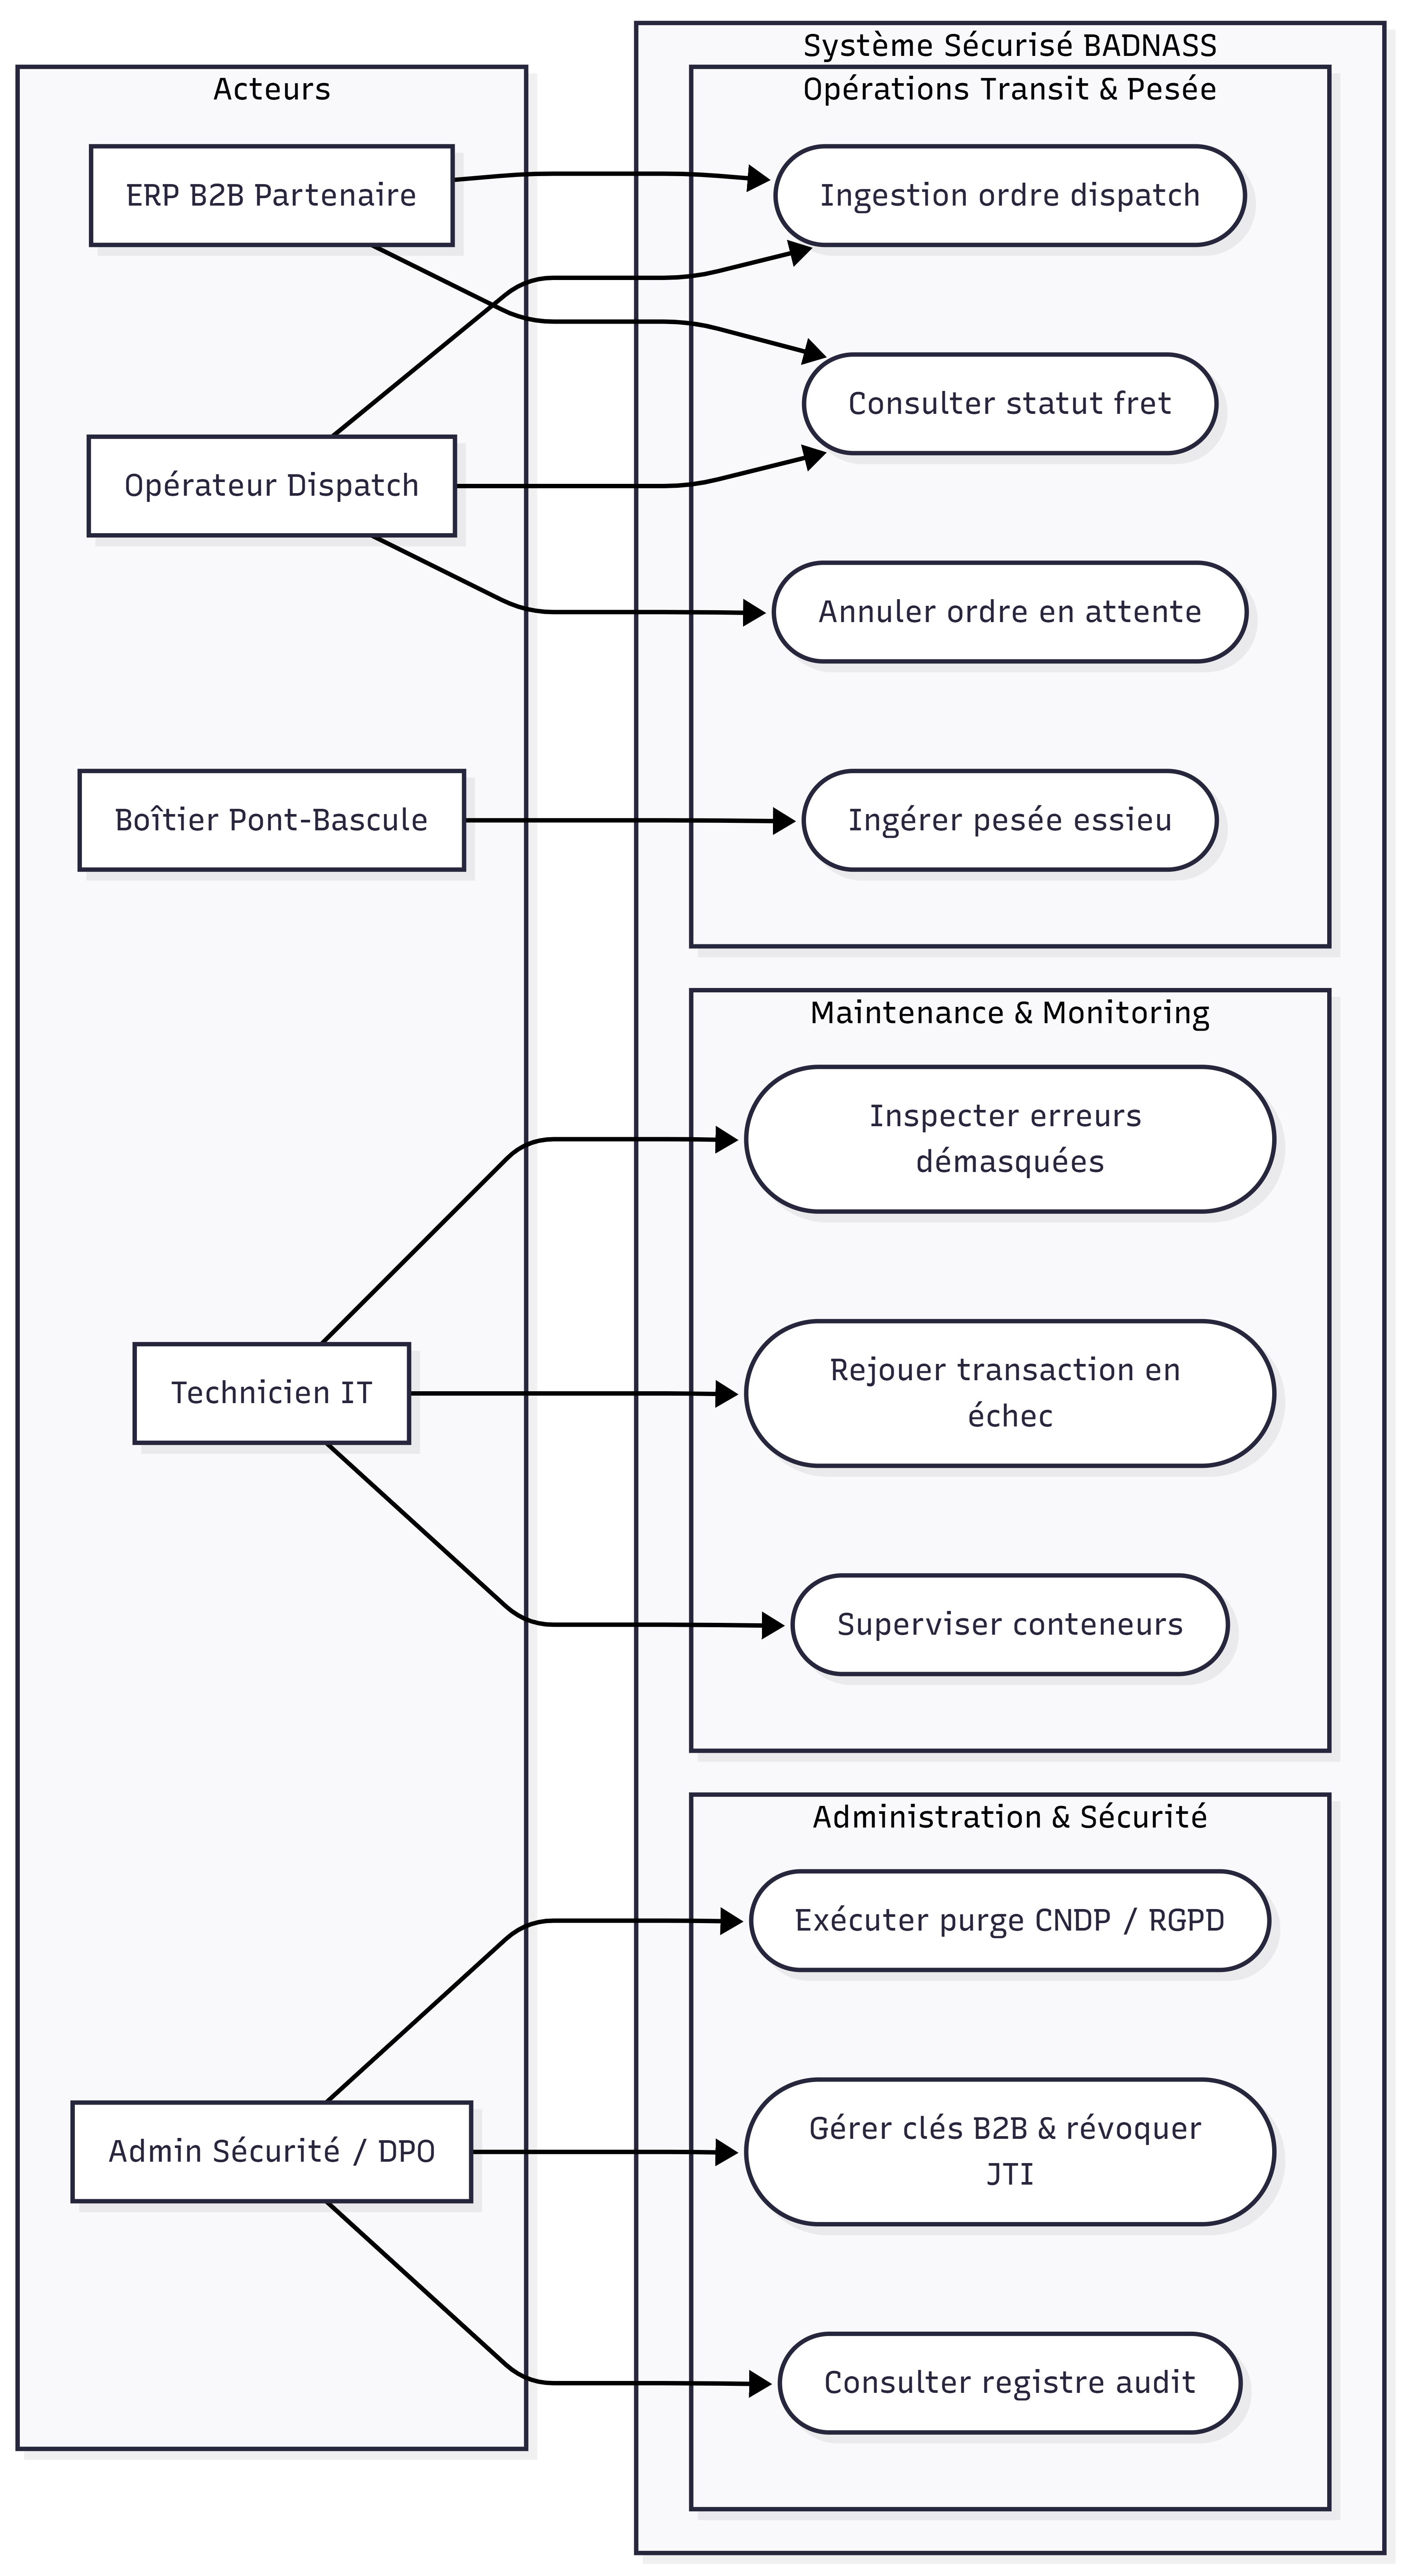
\includegraphics[height=0.68\textheight,keepaspectratio]{figures/uc_diagram.png}
        }{
            \fbox{\parbox[c][0.68\textheight][c]{0.9\linewidth}{\centering \textbf{Figure manquante : figures/uc_diagram.png}}}
        }
        \caption{Diagramme des cas d'utilisation métier — Transitaire Agréé, Déclarant, Opérateur Pont-Bascule et Donneur d'Ordres.}
        \label{fig:uc_diagram}
    \end{figure}
\end{landscape}
\clearpage

% =============================================================================
% 2. DIAGRAMME DU PIPELINE LOGISTIQUE & DONNÉES (PIPELINE DIAGRAM)
% =============================================================================
\begin{landscape}
    \section{Diagramme de Pipeline Logistique \& Flux de Données}
    \vspace{0.5cm}
    \begin{figure}[H]
        \centering
        \IfFileExists{figures/pipeline_diagram.png}{
            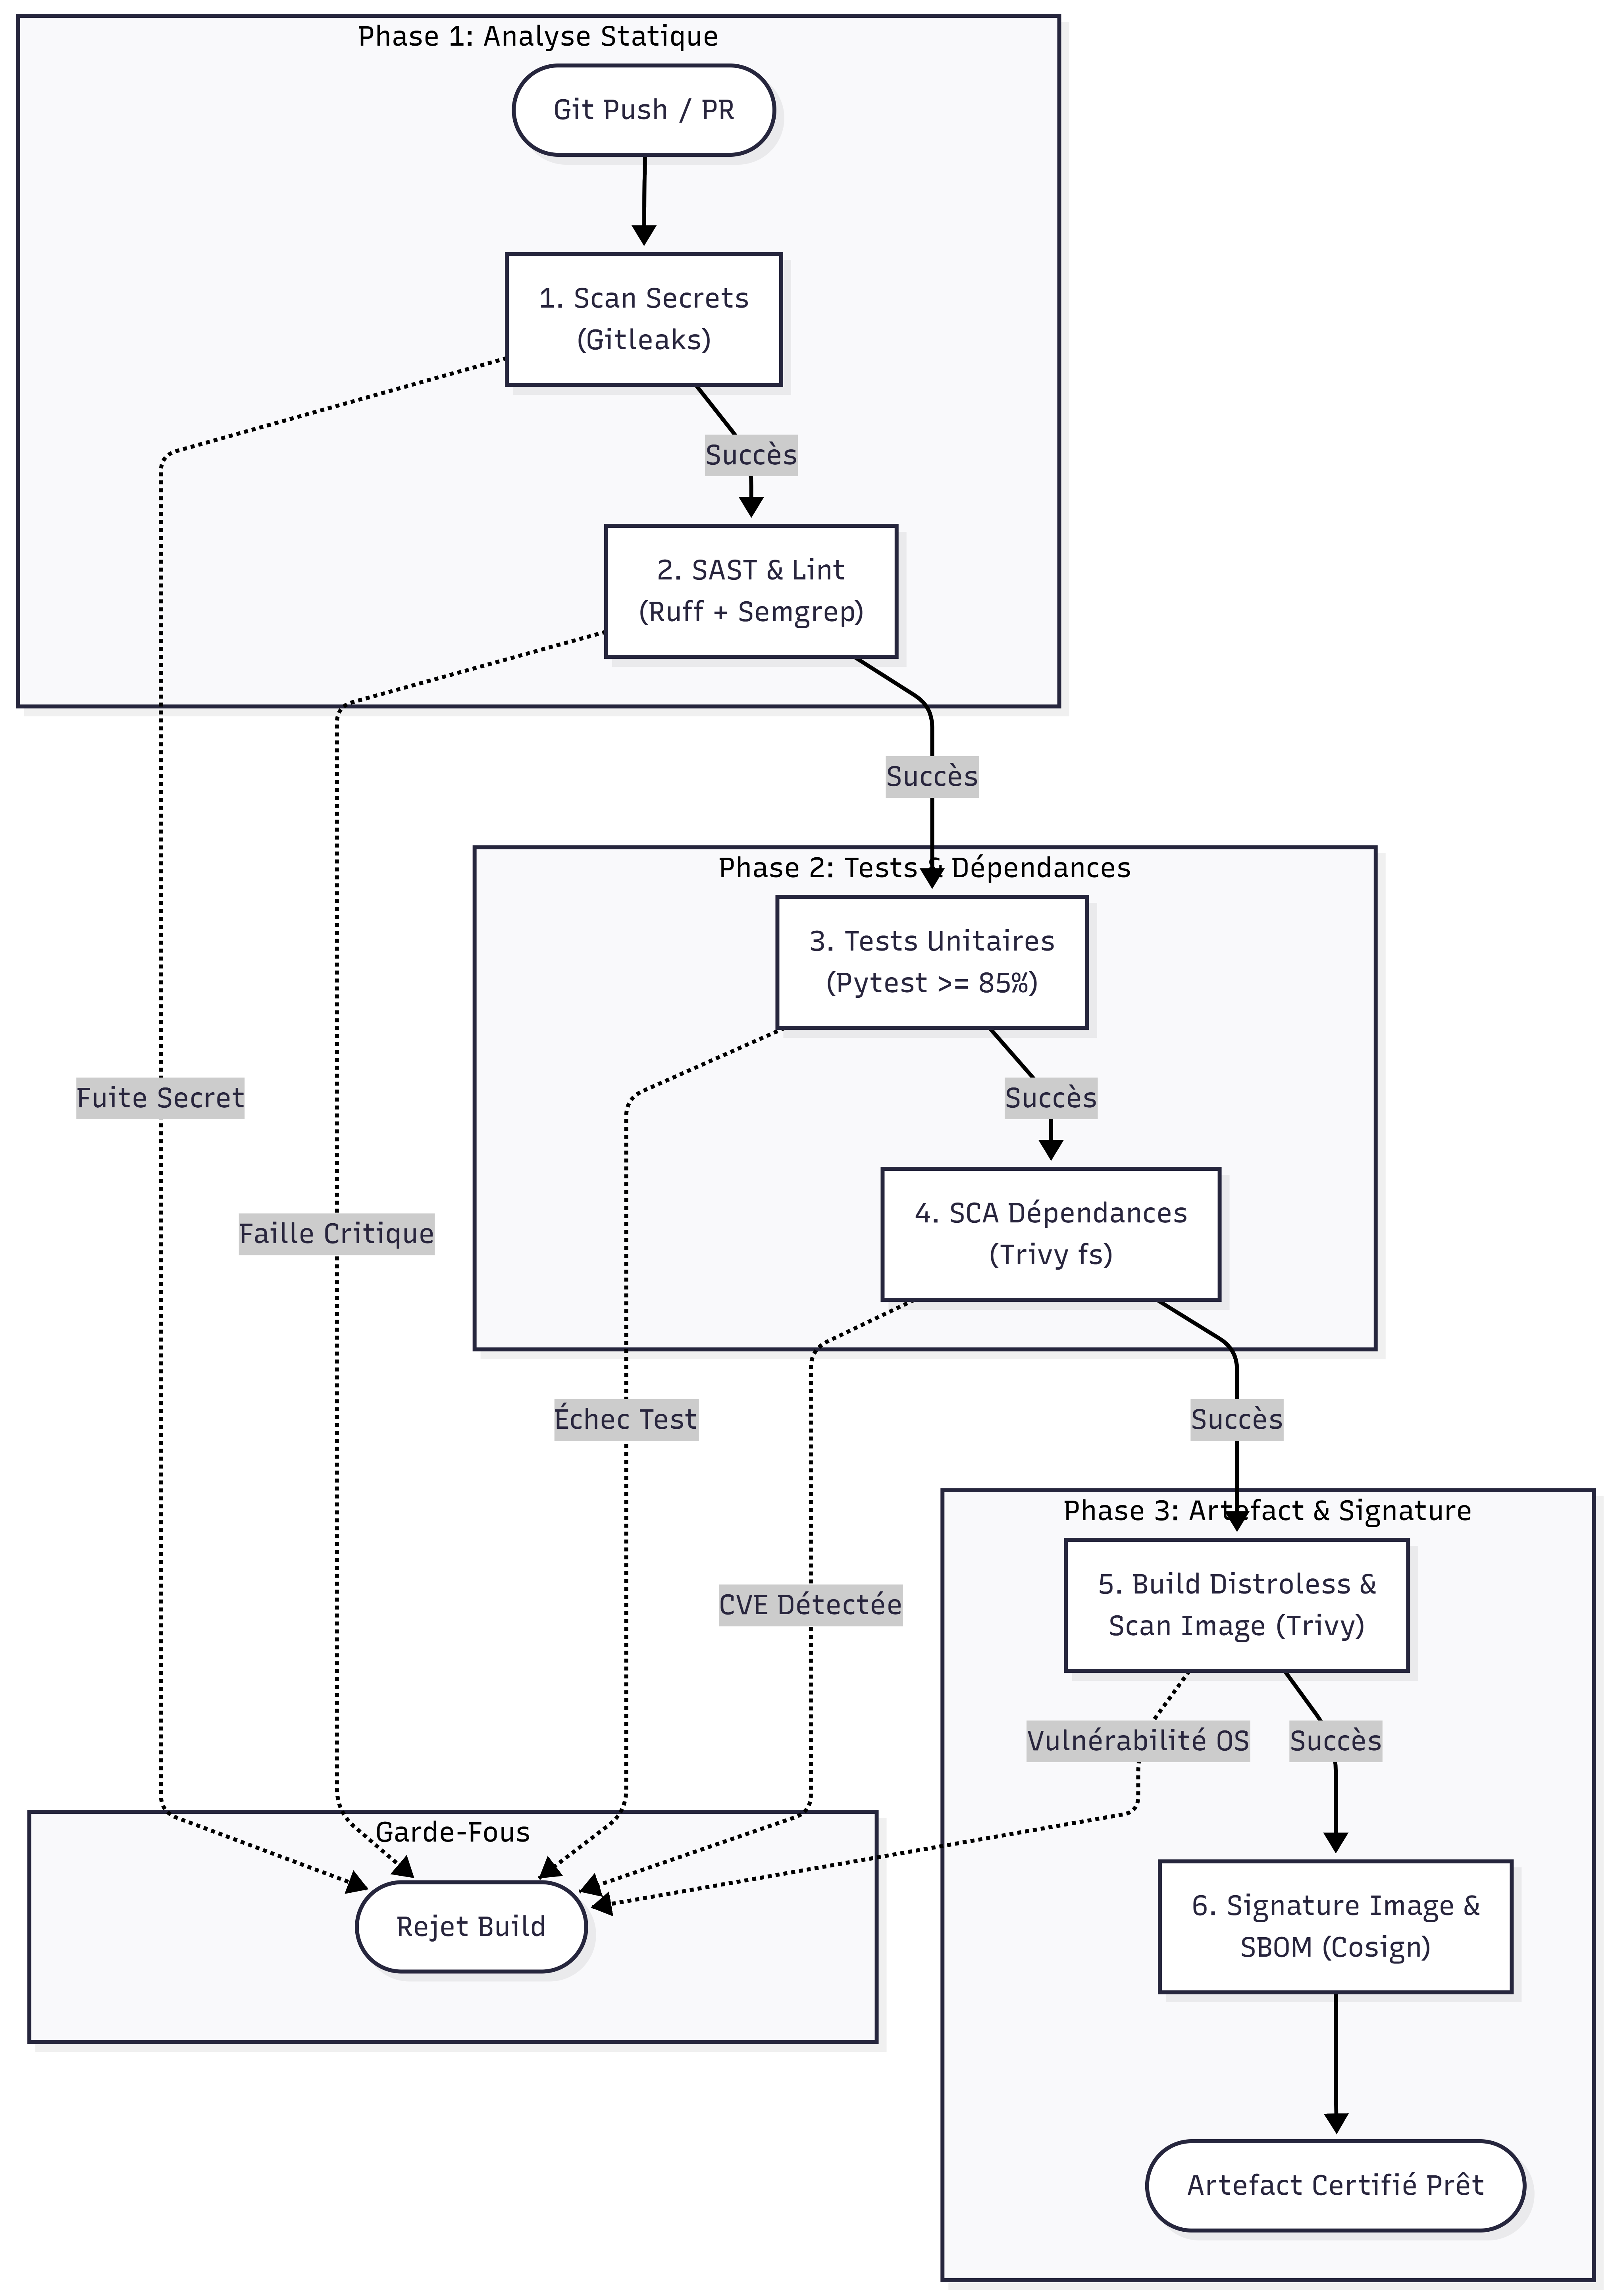
\includegraphics[height=0.68\textheight,keepaspectratio]{figures/pipeline_diagram.png}
        }{
            \fbox{\parbox[c][0.68\textheight][c]{0.9\linewidth}{\centering \textbf{Figure manquante : figures/pipeline_diagram.png}}}
        }
        \caption{Pipeline d'orchestration des flux Import/Export et télétransmission BADR/Portnet.}
        \label{fig:pipeline_diagram}
    \end{figure}
\end{landscape}
\clearpage

% =============================================================================
% 3. GRAPHE DE DÉPENDANCE DES ÉTATS (GDE DIAGRAM)
% =============================================================================
\begin{landscape}
    \section{Graphe de Dépendance des États (GDE Diagram)}
    \vspace{0.5cm}
    \begin{figure}[H]
        \centering
        \IfFileExists{figures/gde_diagram.png}{
            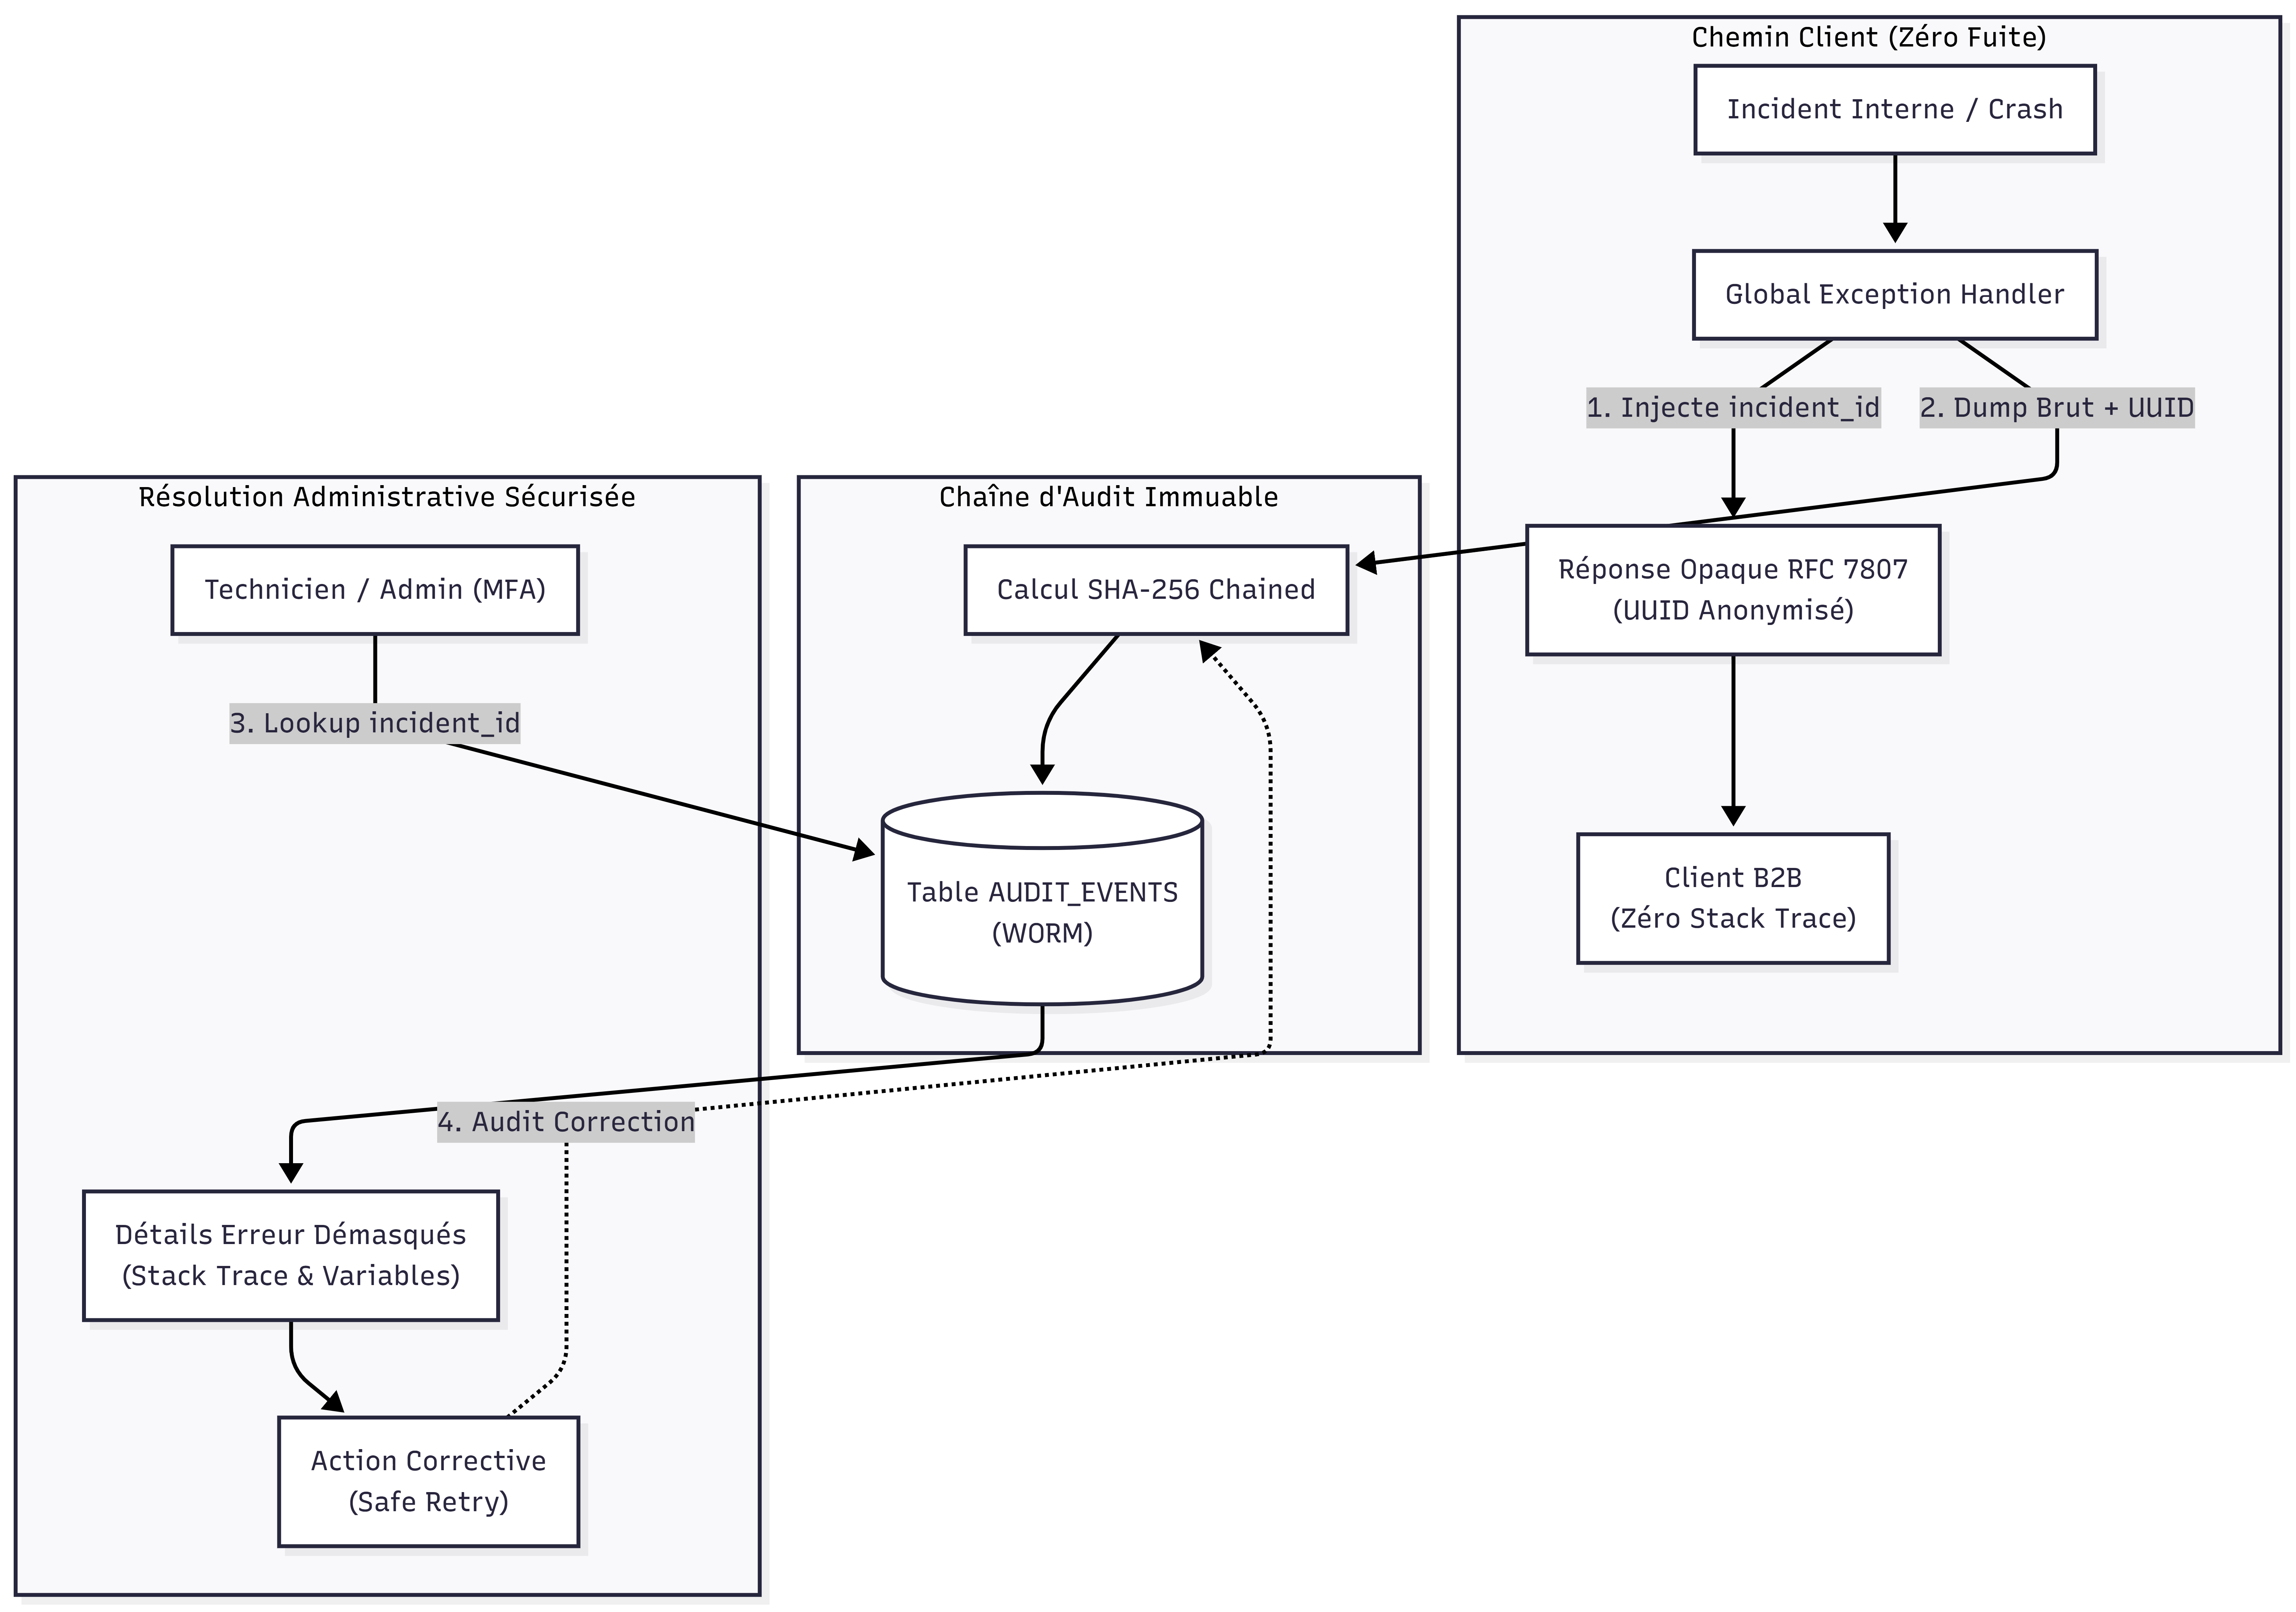
\includegraphics[height=0.68\textheight,keepaspectratio]{figures/gde_diagram.png}
        }{
            \fbox{\parbox[c][0.68\textheight][c]{0.9\linewidth}{\centering \textbf{Figure manquante : figures/gde_diagram.png}}}
        }
        \caption{Automate à états finis du dossier de transit (Enregistrement $\rightarrow$ Contrôle $\rightarrow$ Pesée $\rightarrow$ BAD/Embarqué).}
        \label{fig:gde_diagram}
    \end{figure}
\end{landscape}
\clearpage

% =============================================================================
% 4. MODÈLE ENTITÉ-ASSOCIATION / MODÈLE RELATIONNEL (ERD DIAGRAM)
% =============================================================================
\begin{landscape}
    \section{Diagramme Entité-Relation (ERD Diagram)}
    \vspace{0.5cm}
    \begin{figure}[H]
        \centering
        \IfFileExists{figures/erd_diagram.png}{
            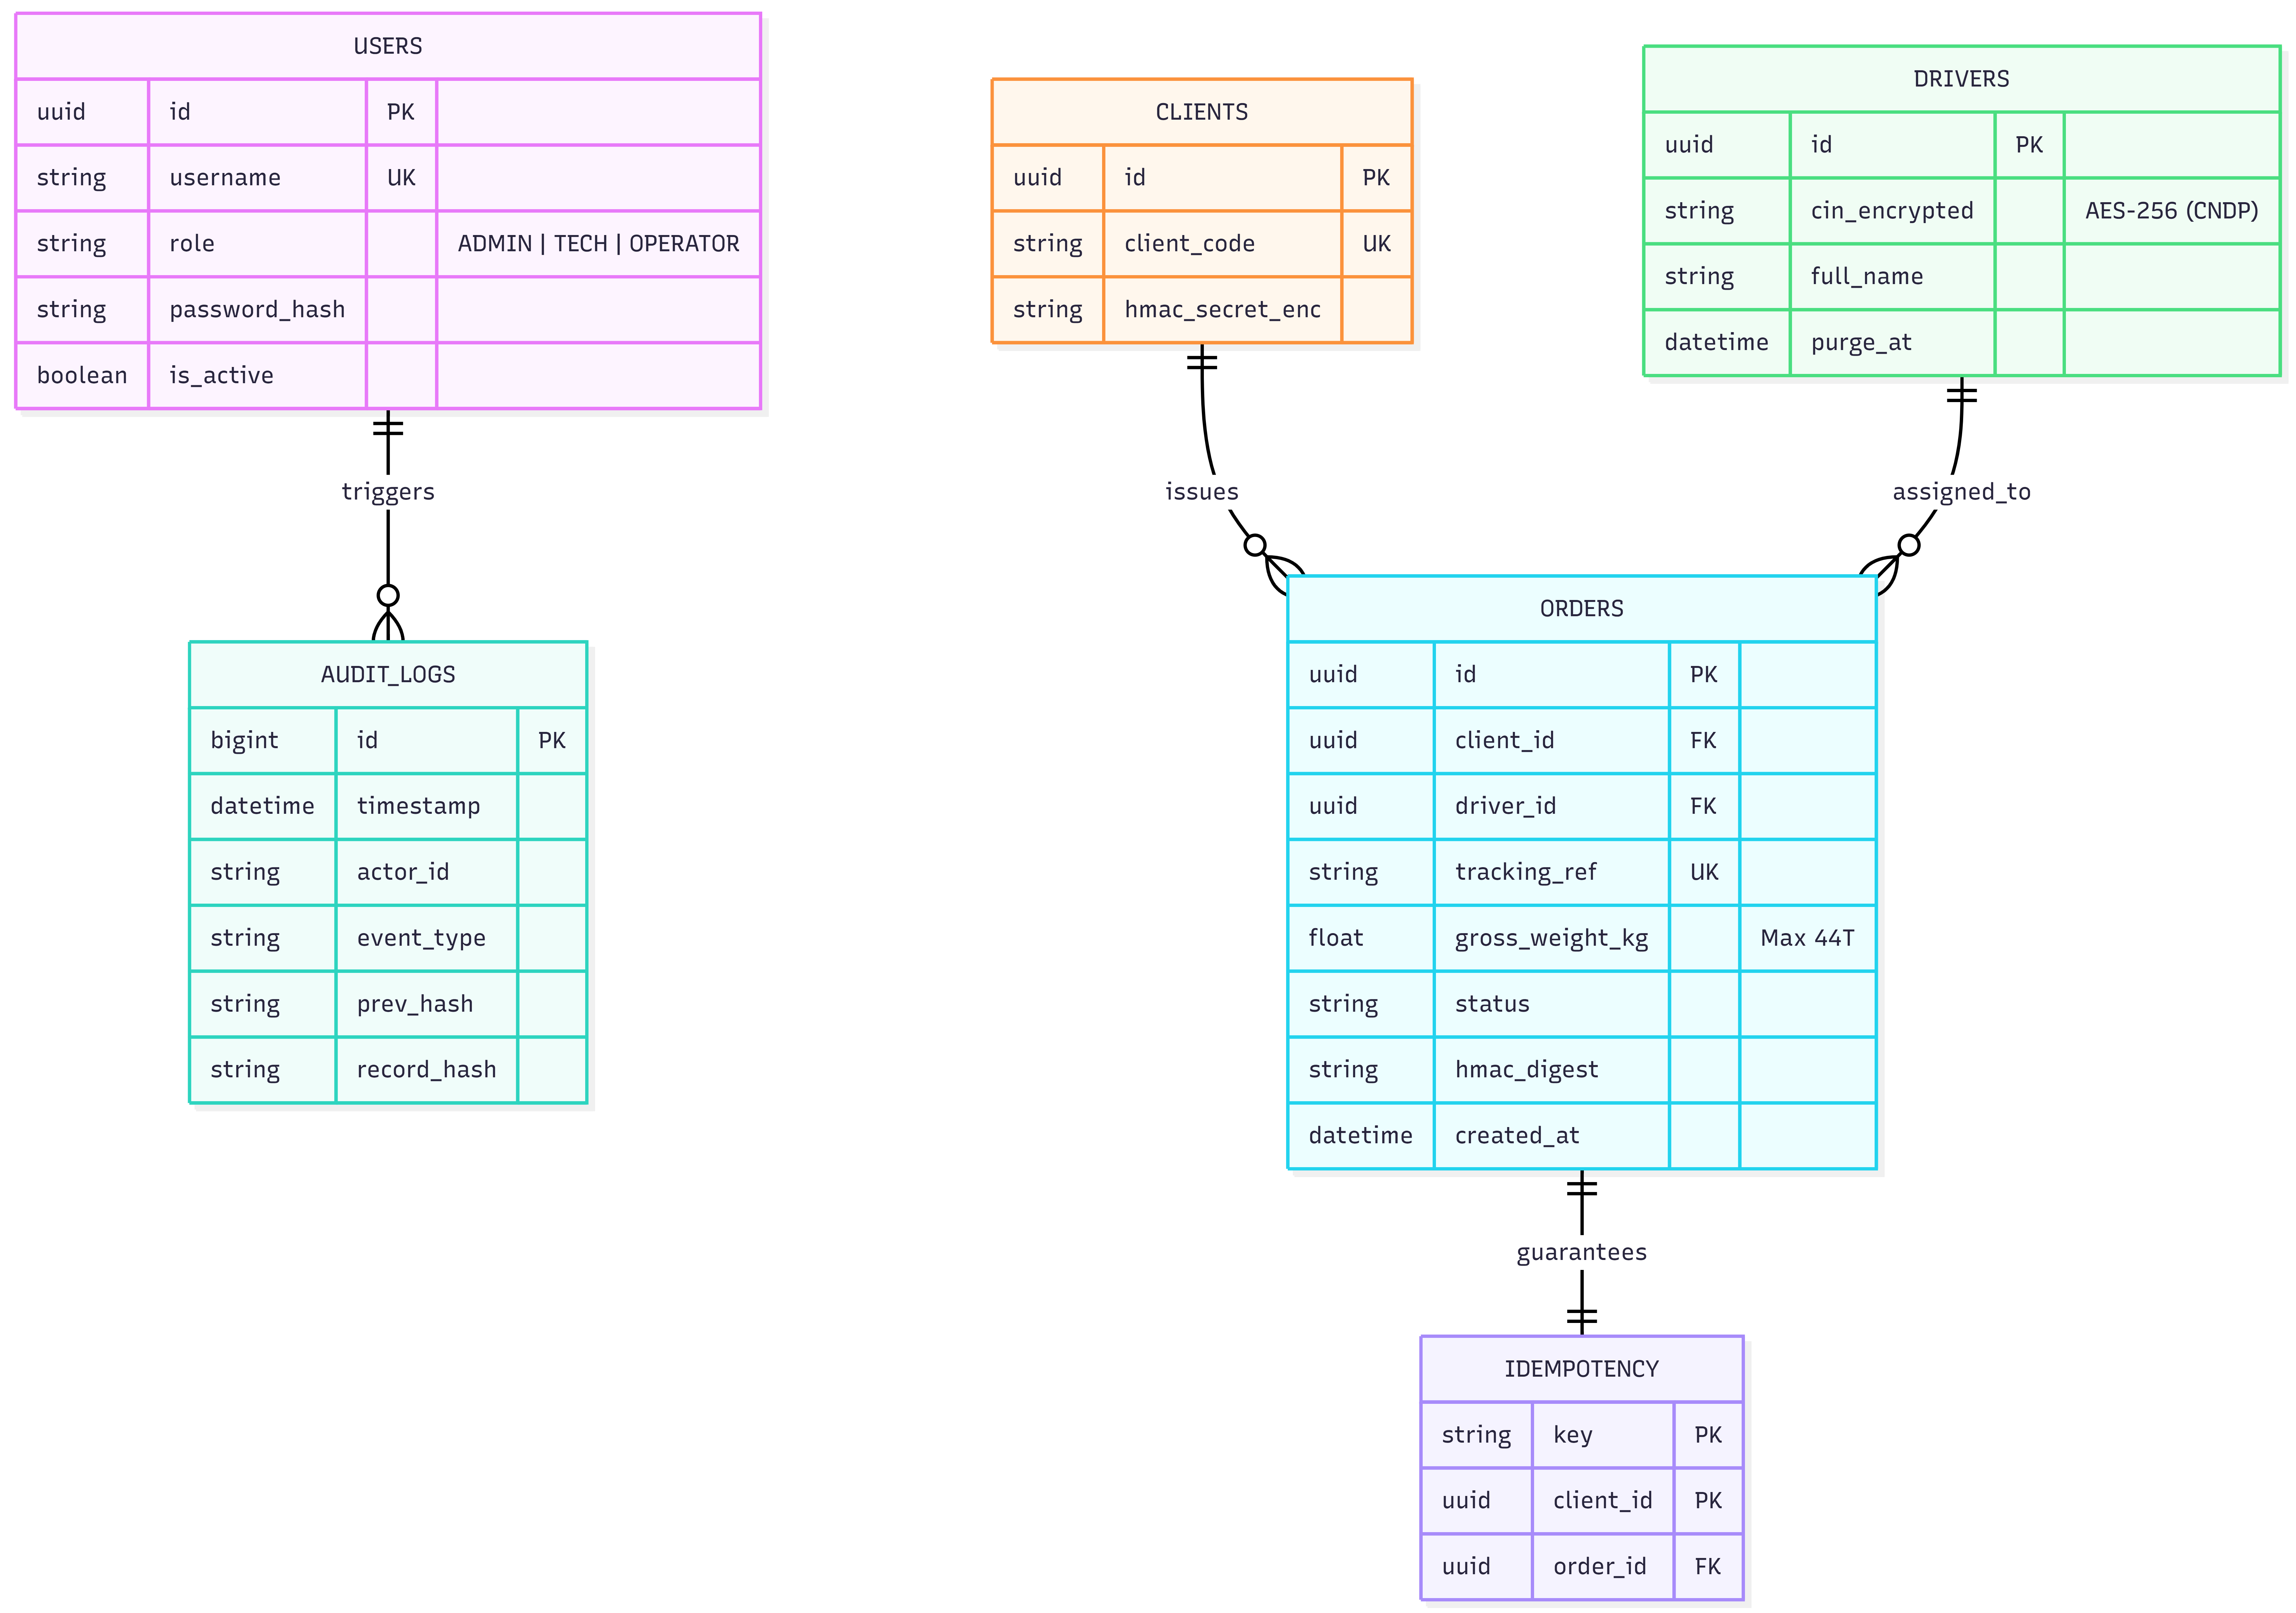
\includegraphics[height=0.68\textheight,keepaspectratio]{figures/erd_diagram.png}
        }{
            \fbox{\parbox[c][0.68\textheight][c]{0.9\linewidth}{\centering \textbf{Figure manquante : figures/erd_diagram.png}}}
        }
        \caption{Modèle logique et relationnel de la base de données opérationnelle BADNASS.}
        \label{fig:erd_diagram}
    \end{figure}
\end{landscape}
\clearpage

% =============================================================================
% 5. DIAGRAMME DE FLUX DE DONNÉES (DFD DIAGRAM)
% =============================================================================
\begin{landscape}
    \section{Diagramme de Flux de Données (DFD Diagram)}
    \vspace{0.5cm}
    \begin{figure}[H]
        \centering
        \IfFileExists{figures/dfd_diagram.png}{
            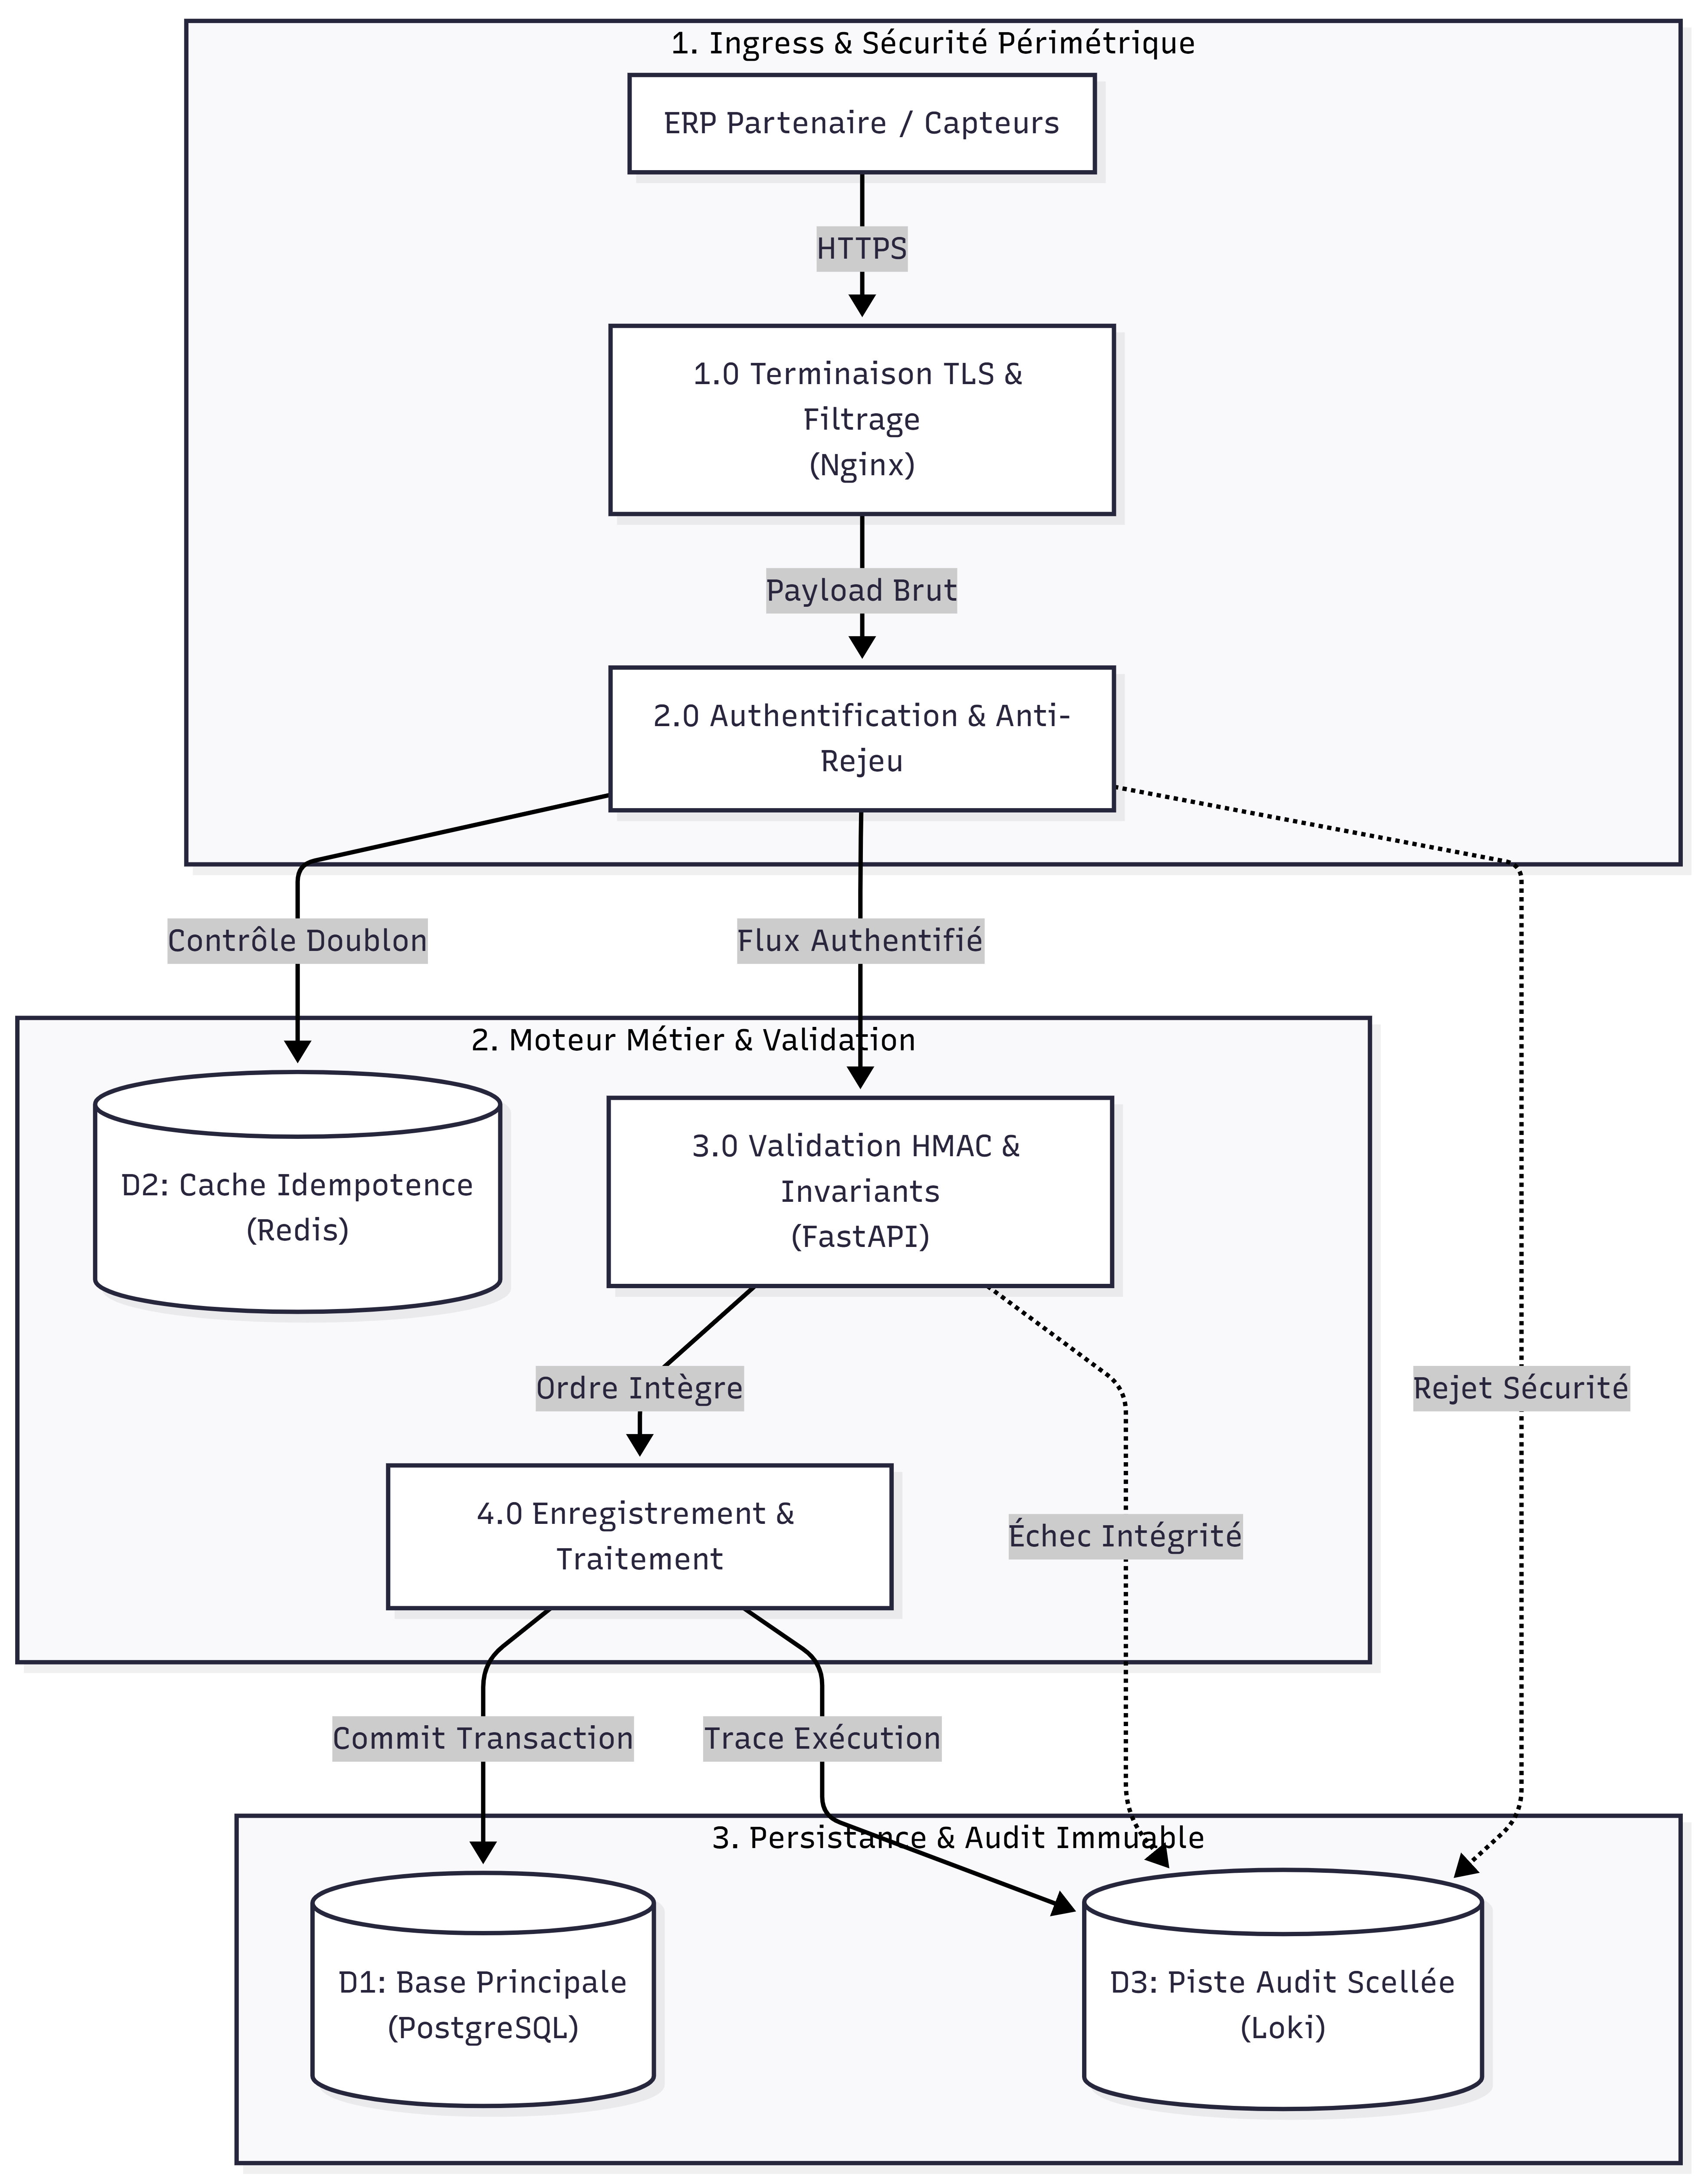
\includegraphics[height=0.68\textheight,keepaspectratio]{figures/dfd_diagram.png}
        }{
            \fbox{\parbox[c][0.68\textheight][c]{0.9\linewidth}{\centering \textbf{Figure manquante : figures/dfd_diagram.png}}}
        }
        \caption{Flux de données sécurisés, signature HMAC et journalisation WORM.}
        \label{fig:dfd_diagram}
    \end{figure}
\end{landscape}
\clearpage

% =============================================================================
% 6. DIAGRAMME DE CLASSES (CLASS DIAGRAM)
% =============================================================================
\begin{landscape}
    \section{Diagramme de Classes Métier (Class Diagram)}
    \vspace{0.5cm}
    \begin{figure}[H]
        \centering
        \IfFileExists{figures/class_diagram.png}{
            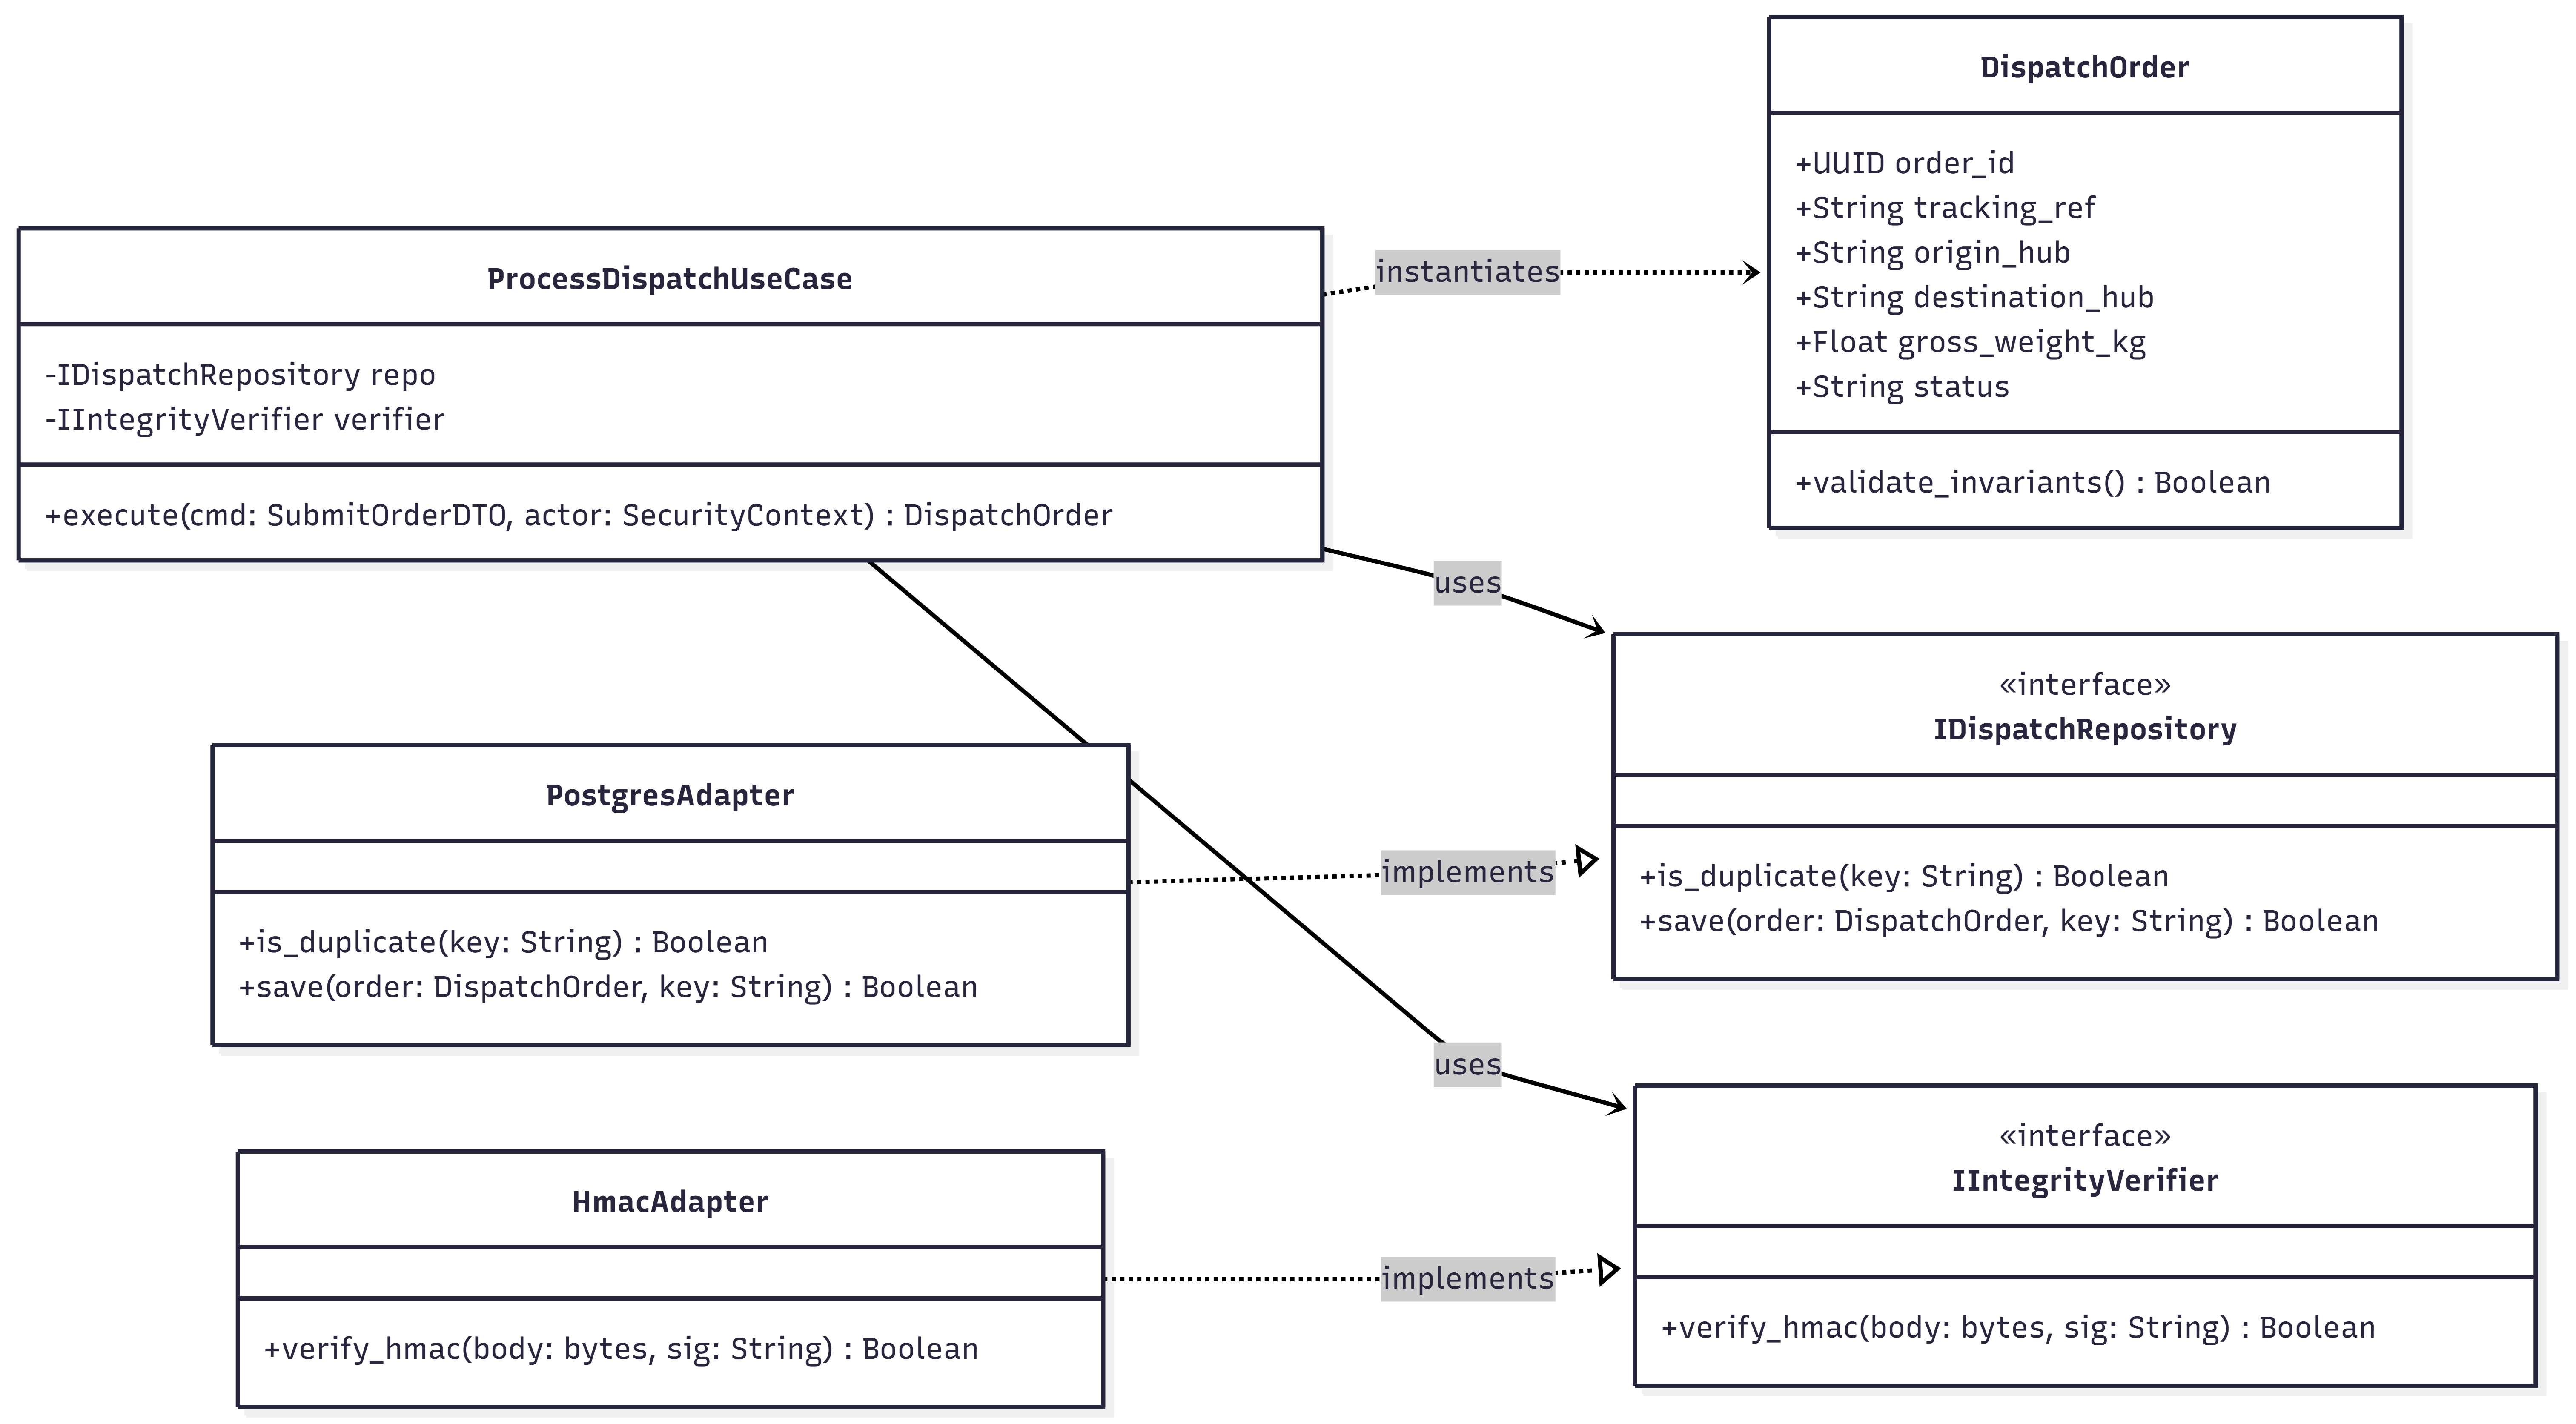
\includegraphics[height=0.68\textheight,keepaspectratio]{figures/class_diagram.png}
        }{
            \fbox{\parbox[c][0.68\textheight][c]{0.9\linewidth}{\centering \textbf{Figure manquante : figures/class_diagram.png}}}
        }
        \caption{Architecture hexagonale — Modèles de domaine, agrégats, ports applicatifs et adaptateurs d'infrastructure.}
        \label{fig:class_diagram}
    \end{figure}
\end{landscape}
\clearpage

% =============================================================================
% 7. DIAGRAMME D'ACTIVITÉ GLOBALE (ACTIVITY DIAGRAM)
% =============================================================================
\begin{landscape}
    \section{Diagramme d'Activité Globale (Activity Diagram)}
    \vspace{0.5cm}
    \begin{figure}[H]
        \centering
        \IfFileExists{figures/ag_diagram.png}{
            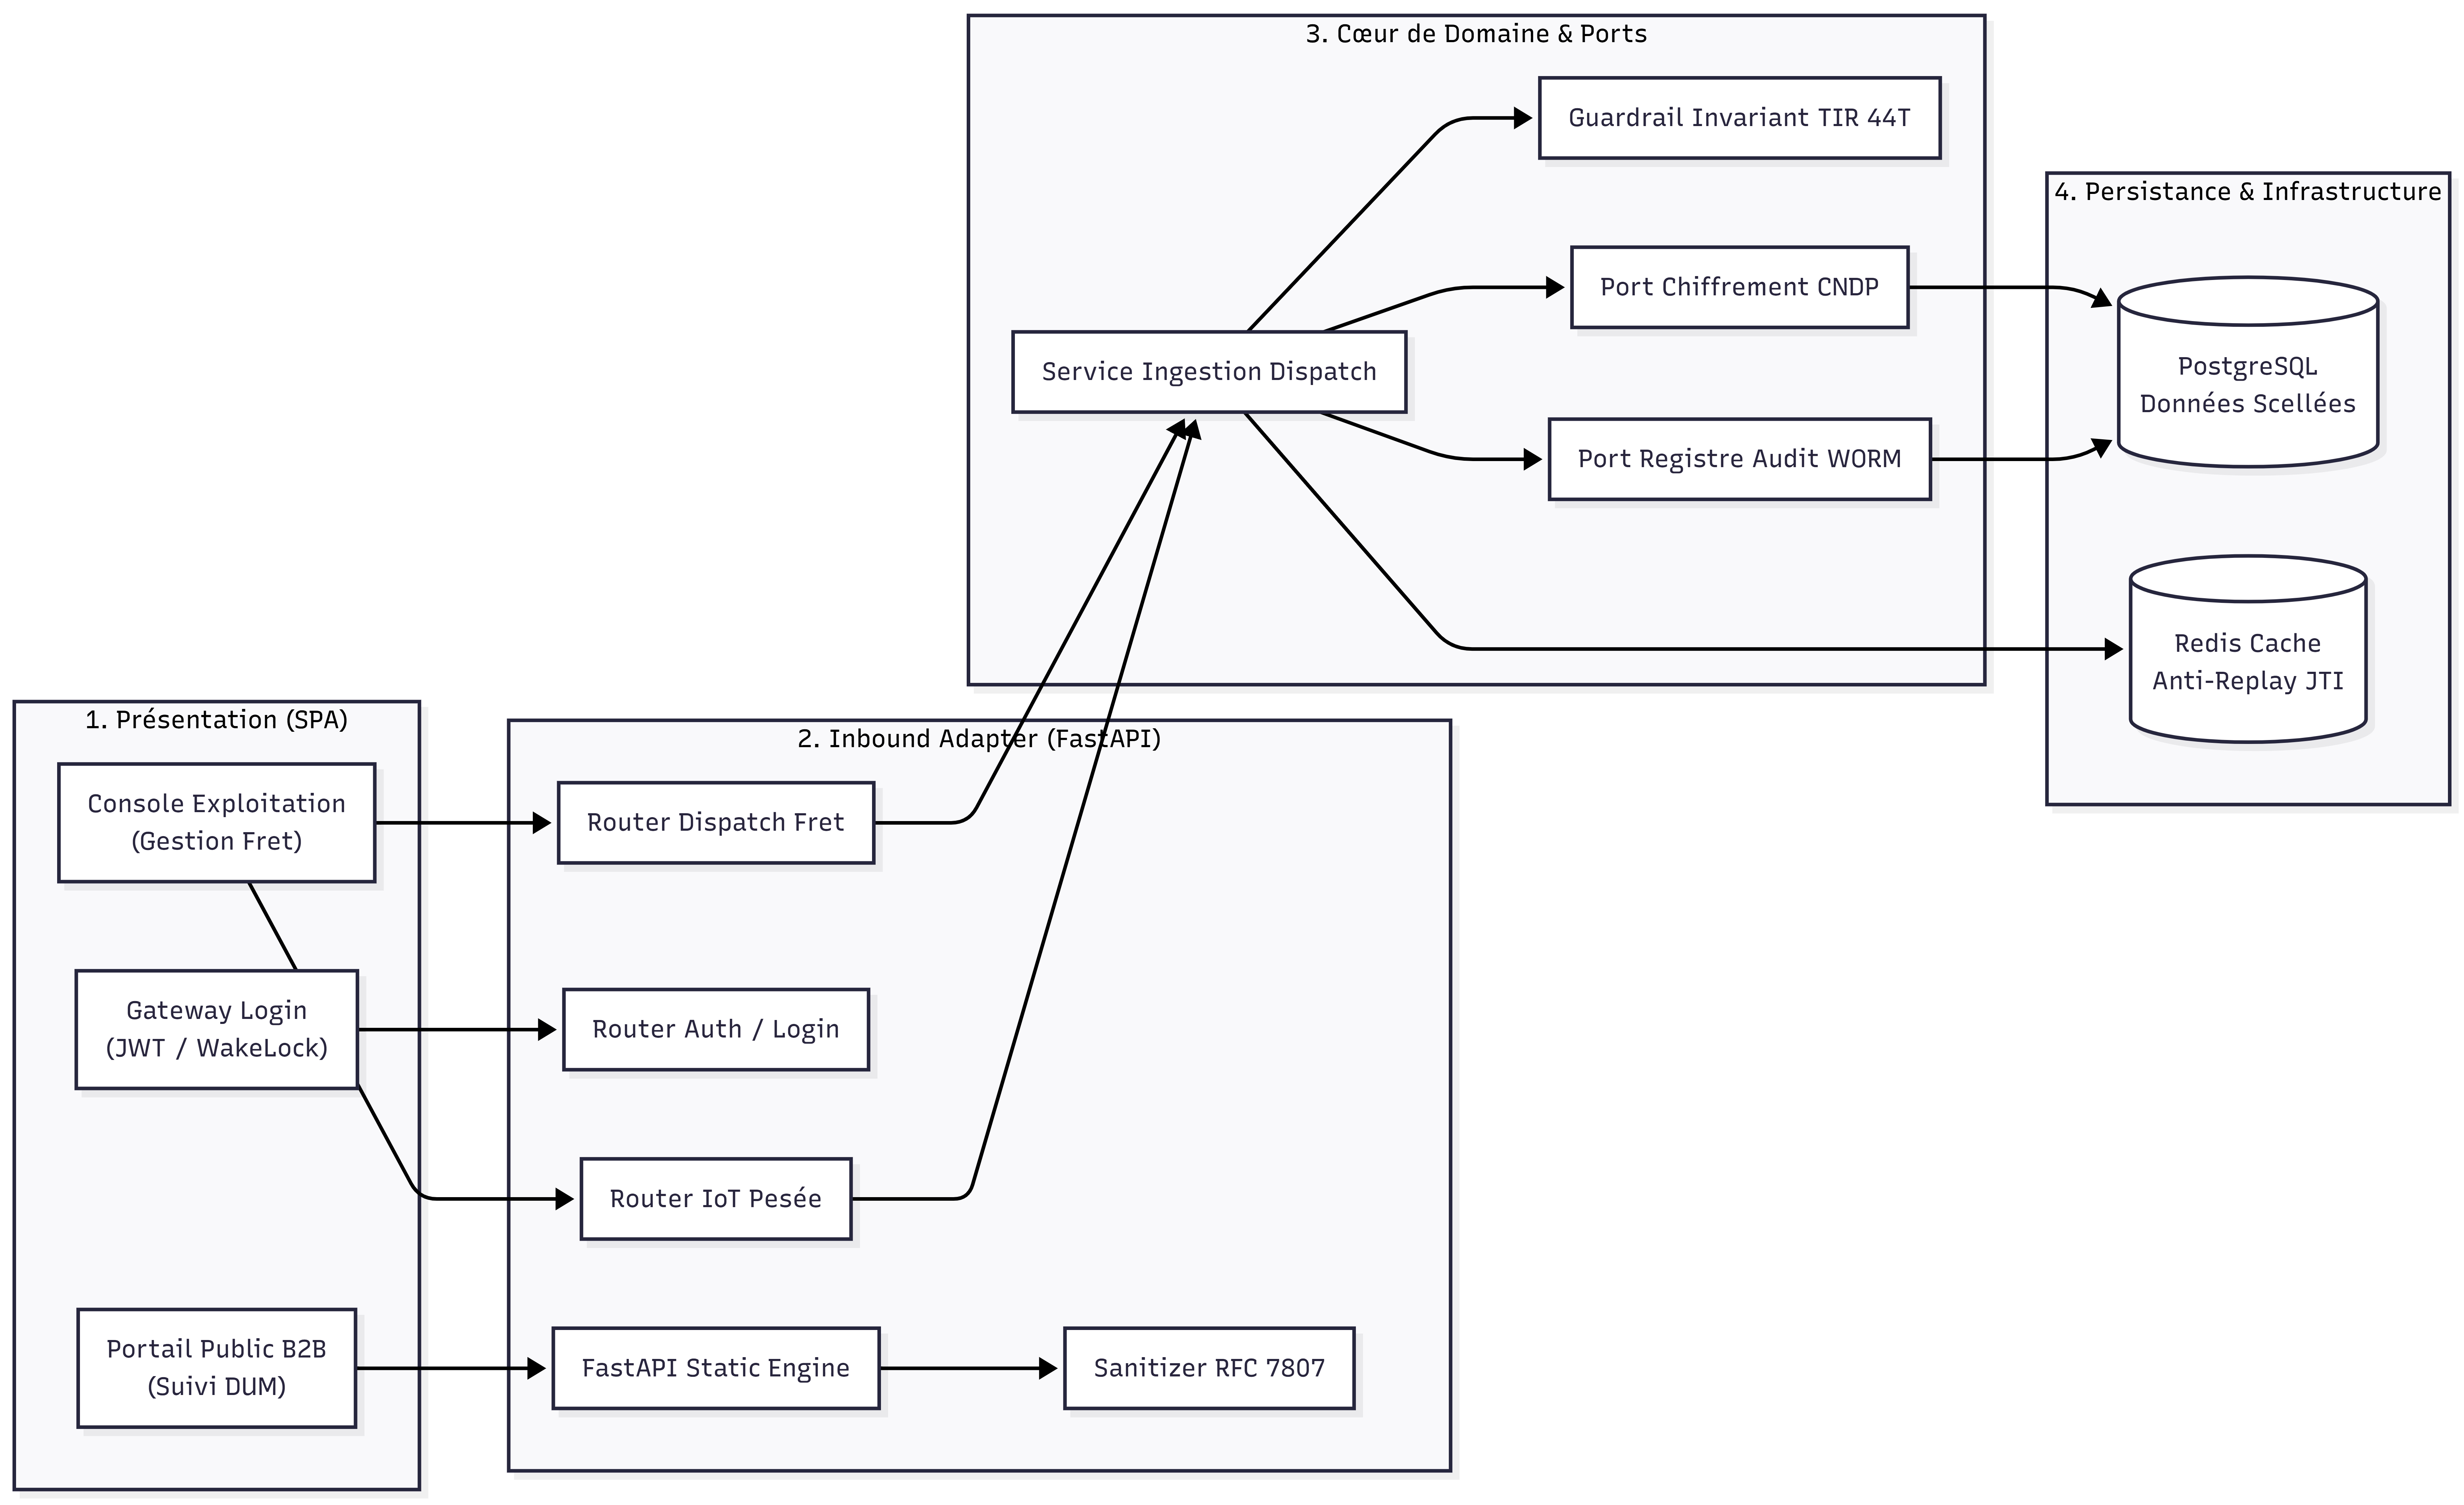
\includegraphics[height=0.68\textheight,keepaspectratio]{figures/ag_diagram.png}
        }{
            \fbox{\parbox[c][0.68\textheight][c]{0.9\linewidth}{\centering \textbf{Figure manquante : figures/ag_diagram.png}}}
        }
        \caption{Déroulement des activités du passage portuaire et garde-fous de conformité TIR 44 Tonnes.}
        \label{fig:ag_diagram}
    \end{figure}
\end{landscape}
\clearpage

% =============================================================================
% 8. DIAGRAMME DE SÉQUENCE SÉCURISÉ (SEQUENCE DIAGRAM)
% =============================================================================
\begin{landscape}
    \section{Diagramme de Séquence Système (Sequence Diagram)}
    \vspace{0.5cm}
    \begin{figure}[H]
        \centering
        \IfFileExists{figures/sequence_diagram.png}{
            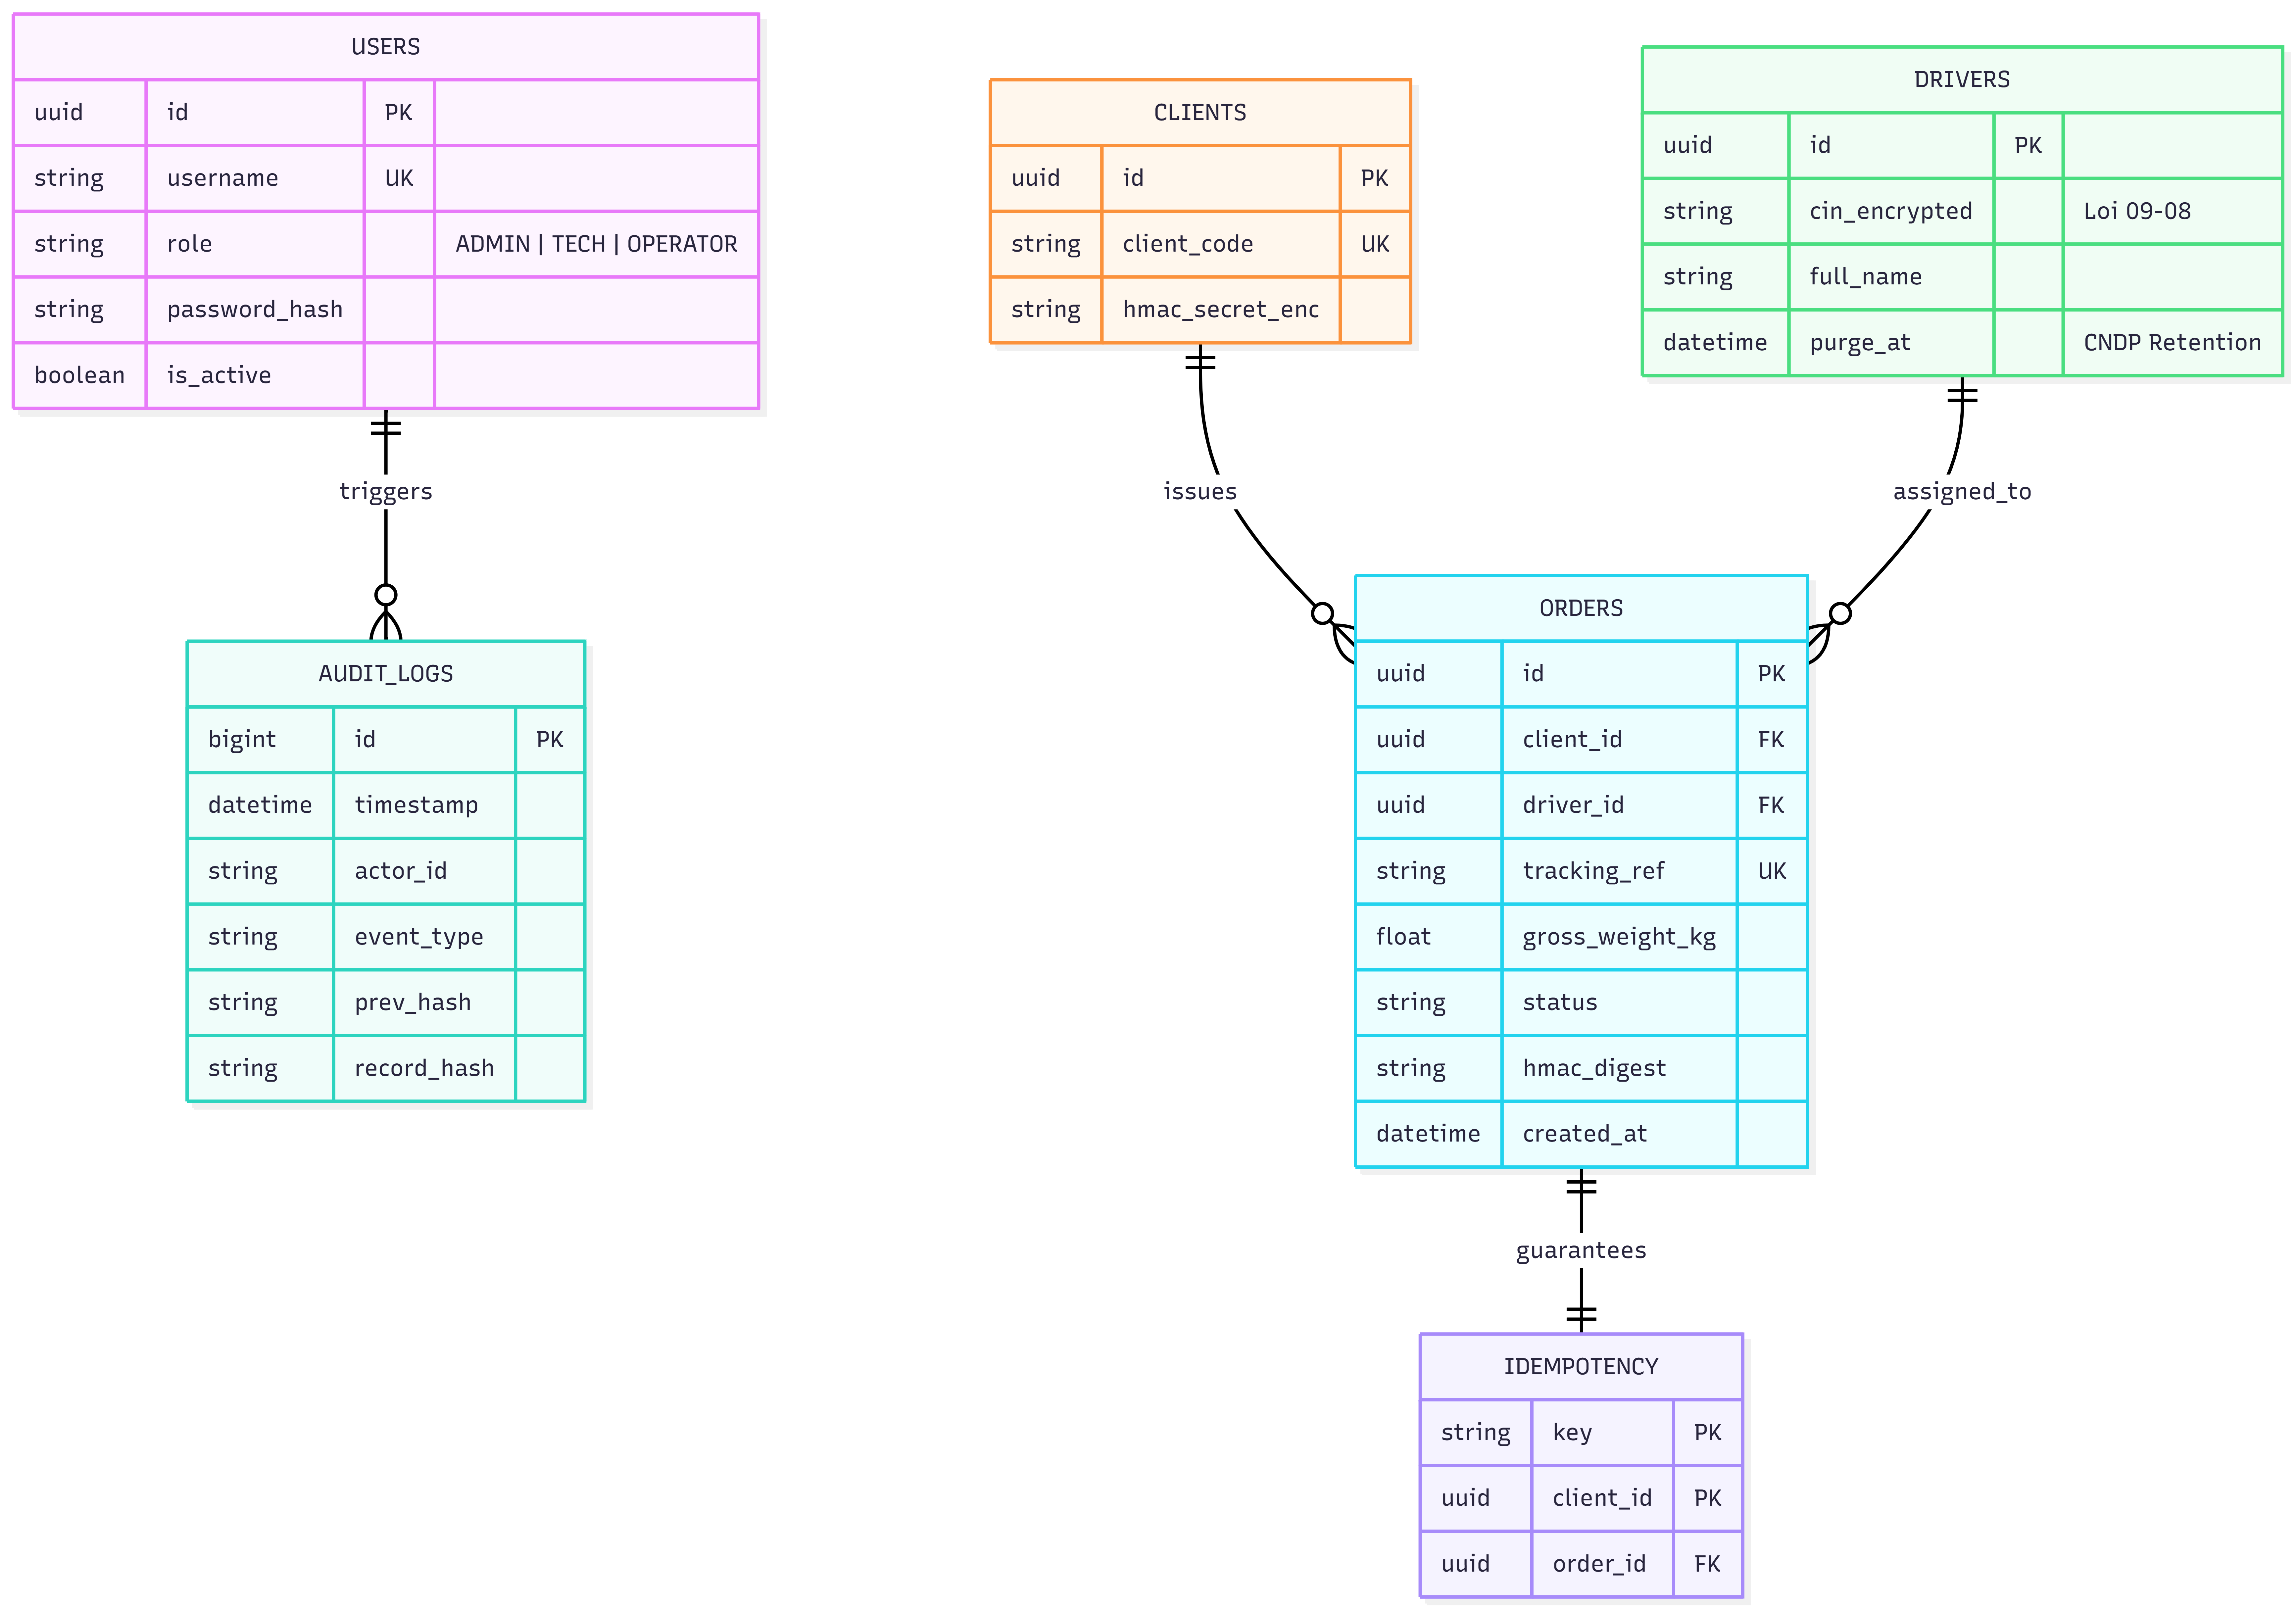
\includegraphics[height=0.68\textheight,keepaspectratio]{figures/sequence_diagram.png}
        }{
            \fbox{\parbox[c][0.68\textheight][c]{0.9\linewidth}{\centering \textbf{Figure manquante : figures/sequence_diagram.png}}}
        }
        \caption{Échanges de messages chiffrés, contrôle anti-rejeu et validation au pont-bascule.}
        \label{fig:sequence_diagram}
    \end{figure}
\end{landscape}
\clearpage

\end{document}
